% AI-VHRS research manuscript -- DRAFT FOR SUPERVISOR REVIEW (not submitted, not peer reviewed).
% All numbers in this file are produced by experiments/runner.py + analysis/analyze.py (see REPRODUCIBILITY.md).
% Author names, affiliations, e-mails and acknowledgements are placeholders to be confirmed by the authors.
\documentclass[conference]{IEEEtran}
\IEEEoverridecommandlockouts
\usepackage[T1]{fontenc}
\usepackage{cite}
\usepackage{amsmath,amssymb,amsfonts}
\usepackage{graphicx}
\usepackage{booktabs}
\usepackage{multirow}
\usepackage{algorithm}
\usepackage{algpseudocode}
\usepackage{xcolor}
\usepackage{url}
\usepackage{tikz}
\usetikzlibrary{arrows.meta,positioning,fit,calc}
\def\BibTeX{{\rm B\kern-.05em{\sc i\kern-.025em b}\kern-.08em T\kern-.1667em\lower.7ex\hbox{E}\kern-.125emX}}
\newcommand{\mm}{\,\mathrm{mm}}
\newcommand{\R}{\mathbb{R}}
\begin{document}

\title{Simulation-Based Evaluation of Two- and Three-Socket MUKCa Kinematic Calibration with Trajectory Pre-Compensation for a Closed-Controller 6-DOF Cobot in Vietnamese Handwriting Reproduction}

\author{\IEEEauthorblockN{[Author 1]\textsuperscript{*}, [Author 2], [Author 3]}
\IEEEauthorblockA{\textit{[Department / Faculty -- to be confirmed by the authors]}\\
\textit{[University -- to be confirmed]}, [City], Vietnam\\
\textsuperscript{*}[corresponding e-mail -- to be confirmed]}
\and
\IEEEauthorblockN{[Supervisor -- to be confirmed]}
\IEEEauthorblockA{\textit{[Affiliation -- to be confirmed]}}}

\maketitle

\begin{abstract}
Collaborative robots are repeatable but not necessarily accurate, and robotic handwriting exposes this gap: a pen that is
a fraction of a millimetre off distorts letter shapes and diacritics. MUKCa recently showed that a 3D-printable two-socket
ball tool suffices to calibrate redundant 7-DOF cobots. We study whether this transfers to the non-redundant 6-DOF FAIRINO
FR3 used in the AI-VHRS Vietnamese handwriting system, whose closed controller cannot accept a corrected kinematic model.
We (i) generalise the MUKCa objective to $K$ sockets with known pairwise distances, (ii) analyse identifiability for the
6-DOF arm, (iii) pre-compensate trajectories by sending the controller the nominal pose of the calibrated joint solution,
and (iv) evaluate everything in a simulation whose ground-truth robots carry geometric deviations plus unmodelled joint
errors and gravity compliance that the calibration never sees. The nominal model was first validated against two
read-only controller readings (flange position within 0.011\,mm). Identifiability analysis gives 21 identifiable parameter
combinations out of 39 for every socket layout and tool-tilt range, so a third socket adds no identifiability.
Over 30 simulated robots, the TCP position RMSE on an independent test set fell from 0.748\,mm (nominal) to 0.109\,mm
(two sockets) and 0.044\,mm (three sockets on a triangle, $-60\%$ vs.\ two sockets, $p<10^{-6}$), at the same 60 samples.
Three collinear sockets gave no gain, and the two-socket tool placed twice performed within 10\% of the triangle,
which shows that the benefit comes from two-dimensional socket spread (a $1.6\times$ higher observability index), not from the
socket count. On ten Vietnamese and geometric writing samples, letter-shape distortion fell from 0.233\,mm
(current practice: nominal model with paper probing) to 0.010\,mm, and absolute in-plane error from 0.80 to 0.15\,mm,
the latter bounded by paper-probing uncertainty. All results are simulated; physical validation on the FR3 is pending.
\end{abstract}

\begin{IEEEkeywords}
kinematic calibration, collaborative robots, identifiability, trajectory pre-compensation, robotic handwriting, simulation
\end{IEEEkeywords}

% =====================================================================================================================
\section{Introduction}
Industrial and collaborative robots are typically specified by their repeatability (e.g., a few hundredths of a millimetre),
while their absolute positioning accuracy, which depends on how well the controller's kinematic model matches the physical
arm, can be one to two orders of magnitude worse \cite{nubiola2013,hollerbach1996}. Kinematic calibration closes this gap
by identifying the geometric parameters of the arm from measurements \cite{everett1987,zhuang1992,hollerbach1996}, but
classical procedures rely on laser trackers or coordinate measuring machines that may cost more than a cobot
\cite{nubiola2013,franzese2026mukca}. MUKCa \cite{franzese2026mukca,franzese2025arxiv} removes this barrier: a
3D-printable tool with two sockets constrains the robot's ball-tipped end effector, and an optimisation makes the
predicted ball centre consistent within each socket while preserving the known socket distance. On Franka cobots it reduced
the mean absolute error from about 10\,mm to 0.2\,mm \cite{franzese2026mukca}.

AI-VHRS (AI-Assisted Vietnamese Handwriting Reproduction System) writes cards and letters with a 6-DOF FAIRINO FR3 cobot.
Vietnamese script stacks diacritics (breve, circumflex, horn plus five tone marks) within a few millimetres, so
sub-millimetre geometric errors are visible. Two properties of this application complicate a direct transfer of MUKCa.
First, MUKCa assumes a kinematically redundant arm, whose null-space motion produces many distinct configurations for one
socket \cite{franzese2026mukca}; the FR3 is non-redundant, and with the ball pinned in a socket only the tool orientation
can vary. Second, the FR3 controller is closed: it solves inverse kinematics with its own nominal model, so a calibrated
model cannot be installed and must instead be exploited by modifying the commanded targets.

\textbf{Research questions.} RQ1: How much can socket-based calibration reduce the positioning error of a simulated 6-DOF
cobot? RQ2: Under which conditions does a three-socket configuration measurably outperform the two-socket baseline? RQ3: How
much does calibrated trajectory pre-compensation improve handwriting accuracy under geometric and measurement uncertainty?

\textbf{Contributions.} (1) An identifiability analysis of the MUKCa formulation on a non-redundant 6-DOF arm, showing that
the identifiable rank (21 of 39) matches the classical count for position-only, base-free measurements and does not depend on
socket count or tilt range. (2) A $K$-socket generalisation of the MUKCa objective and a controlled comparison, at equal
sample budgets, of two-socket, collinear three-socket, triangular three-socket and two-placement designs, together with an
explanation of the observed differences via an observability index and a regularisation ablation. (3) A closed-controller
pre-compensation scheme with paper-frame registration, evaluated end-to-end on Vietnamese handwriting trajectories produced
by the AI-VHRS pipeline. (4) A reproducible simulation framework whose ground truth includes errors outside the calibrated
model class, with the nominal model validated against the real controller. We do not claim the three-socket idea itself as
new: MUKCa already mentions more sockets and multiple tool placements as alternatives \cite{franzese2026mukca}; our
contribution is the quantitative evidence of when and why they matter for a 6-DOF closed-controller arm.

% =====================================================================================================================
\section{Related Work}
\textit{Kinematic calibration.} Model-based calibration identifies a complete, minimal set of geometric parameters; for a
serial arm with $R$ revolute and $P$ prismatic joints a complete model has $4R+2P+6$ independent parameters
\cite{everett1987,zhuang1992}. Identifiability and the choice of measurement poses are characterised by the singular values
of the identification Jacobian \cite{borm1991,hollerbach1996}. External metrology (laser trackers, optical CMMs)
\cite{nubiola2013} and newer error models \cite{kim2024,alam2022} give the highest accuracy but need expensive equipment;
open tools such as \cite{pascal2023} lower the software barrier.

\textit{Constraint-based and low-cost calibration.} Closed-loop methods replace the external sensor by geometric
constraints: distance and sphere constraints \cite{joubair2015}, a telescoping ballbar \cite{nubiola2014ballbar}, kinematic
couplings under impedance control \cite{nadeau2019}, an affordable 3D measuring device \cite{gaudreault2018}, and closed
kinematic chains on a redundant cobot \cite{petric2023}. MUKCa \cite{franzese2026mukca} is the most minimal of these: a
printed ball-and-socket tool, consistency plus distance terms, validated on Franka, KUKA and Kinova cobots, with an open
implementation \cite{mukcacode}. Its stated assumptions include kinematic redundancy and negligible joint-angle error.

\textit{Error compensation.} When the controller's model cannot be modified, identified errors are compensated by modifying
targets (``offline'' or ``model-based'' compensation) \cite{nubiola2013,liao2023,alam2022}. We use the joint-space form of
this idea, which is exact for a perfect calibrated model.

\textit{Robotic drawing and handwriting.} Robot portrait drawing \cite{lin2009,nasrat2023} and robotic calligraphy
\cite{guo2025} focus on stroke generation and pen or brush control; to our knowledge these works do not address absolute
kinematic accuracy or low-cost calibration of the arm, which is the gap addressed here for Vietnamese handwriting.

% =====================================================================================================================
\section{Problem Formulation}
\subsection{Kinematic model}
Following the URDF parameterisation used by MUKCa, joint $i$ has a fixed origin transform $T_o(\boldsymbol\theta_i)$ with
$\boldsymbol\theta_i=(x_i,y_i,z_i,\phi_i,\vartheta_i,\psi_i)$ (translation in mm, roll--pitch--yaw in rad) followed by a
rotation $q_i$ about its local $z$ axis. The tool-centre point (TCP) is
\begin{equation}
\mathbf{f}_{\boldsymbol\theta}(\mathbf q)=\mathbf{p}\Big(\prod_{i=1}^{6}T_o(\boldsymbol\theta_i)\,R_z(q_i)\;
T(\mathbf t)\Big),\label{eq:fk}
\end{equation}
where $\mathbf t$ is the tool offset and $\mathbf p(\cdot)$ extracts the translation. With the ball offset,
$\boldsymbol\theta\in\R^{39}$ (36 joint-origin parameters and 3 ball-offset parameters). Joint zero offsets are contained in
the yaw parameters. Nominal values come from the vendor URDF \cite{frcoburdf}.

\subsection{Socket measurement equations}
$K$ sockets with unknown positions $\mathbf s_k$ are fixed on the table; a subset $\mathcal D$ of socket pairs lies on one
rigid tool, so their distances $d_{kl}$ are known (caliper-measured). For each socket, $N_k$ configurations are recorded
while the ball sits in it:
\begin{equation}
\mathbf f_{\boldsymbol\theta^\star}(\tilde{\mathbf q}_{ki}) = \mathbf s_k + \boldsymbol\epsilon^{\rm seat}_{ki},\qquad
\mathbf q_{ki}=\tilde{\mathbf q}_{ki}+\boldsymbol\epsilon^{q}_{ki},\label{eq:meas}
\end{equation}
where $\boldsymbol\theta^\star$ is the (unknown) true geometry, $\tilde{\mathbf q}$ the true joint angles and $\mathbf q$ the
encoder readings. On the real robot, $\boldsymbol\theta^\star$ is only an approximation of the arm: compliance and transmission
errors are not part of (\ref{eq:fk}).

\subsection{Calibration objective}
Let $\boldsymbol\mu_k(\boldsymbol\theta)=\frac{1}{N_k}\sum_i\mathbf f_{\boldsymbol\theta}(\mathbf q_{ki})$ and
$N=\sum_k N_k$. Generalising MUKCa (Eq.~5 of \cite{franzese2026mukca}) from two sockets to $K$ sockets:
\begin{align}
J(\boldsymbol\theta)&=\frac1N\sum_{k=1}^{K}\sum_{i=1}^{N_k}\big\|\mathbf f_{\boldsymbol\theta}(\mathbf q_{ki})-\boldsymbol\mu_k\big\|^2\nonumber\\
&+\!\!\sum_{(k,l)\in\mathcal D}\!\!\big(\|\boldsymbol\mu_k-\boldsymbol\mu_l\|-d_{kl}\big)^2
+\lambda\|\boldsymbol\theta-\boldsymbol\theta_{\rm nom}\|^2 .\label{eq:J}
\end{align}
The first term is the sample-weighted trace of the per-socket covariance (consistency), the second preserves the known
distances (distortion), and the third keeps the solution near the nominal model. In mm/mrad units, $\lambda=10^{-4}$ is
equivalent to MUKCa's $\lambda=10^{-4}$ in m/rad units. No socket position $\mathbf s_k$ in the base frame enters
(\ref{eq:J}), so a rigid motion of the base frame leaves $J$ unchanged (a 6-dimensional gauge freedom).

\subsection{Identifiability}
Let $\mathbf J_r=\partial\mathbf r/\partial\boldsymbol\theta$ be the Jacobian of the consistency and distance residuals
at a zero-residual point (noise-free data, model inside the model class). Its numerical rank $r$ (singular values
$\sigma_i>10^{-6}\sigma_1$) is the number of identifiable parameter combinations, and we use the geometric mean of the
identifiable singular values, $O_1=(\prod_{i=1}^{r}\sigma_i)^{1/r}$, as an observability index in the spirit of
\cite{borm1991}. For a 6R arm, the complete-model count $4R+6=30$ \cite{everett1987,zhuang1992}, minus 3 tool-orientation
parameters that position-only data cannot see and minus the 6 base gauge parameters, predicts $r=21$.

\subsection{Error definitions}
Errors are evaluated against the simulated ground truth in four spaces, which we keep separate. (a) \emph{Model-space TCP
error} (E1): $e_j=\|R\,\mathbf f_{\hat{\boldsymbol\theta}}(\mathbf q_j)+\mathbf b-\mathbf f^\star(\tilde{\mathbf q}_j)\|$ on an
independent test set, after the best rigid alignment $(R,\mathbf b)$ (Kabsch), which removes the gauge; raw errors are
also reported. (b) \emph{Paper-space error} (E5): the true pen tip is expressed in the true paper frame
$(u,v,h)$; the in-plane error is $e_i=\|(u_i,v_i)-(u_i^{d},v_i^{d})\|$ and $h_i$ is the height above the sheet.
(c) \emph{Shape error}: $e_i$ after the best 2-D rigid fit of the executed points of one sample onto the desired ones,
i.e., letter-shape distortion with the sheet-registration offset removed. (d) \emph{Real ink-on-paper quality} is not
simulated; contact ratio $\Pr(h_i<p)$ for a commanded press depth $p$ is only a geometric proxy.

% =====================================================================================================================
\section{Proposed Methodology}
\subsection{Three-socket adaptation}
We place three sockets on the vertices of an equilateral triangle with side $d$ on the writing table, so that (\ref{eq:J})
contains three distance terms and the socket set spans the writing plane. As controls we use (i) the MUKCa two-socket tool
(S2), (ii) three collinear sockets (S3L: same count, no 2-D spread) and (iii) the two-socket tool at two placements, along $x$
and along $y$ (S2$\times$2), which MUKCa supports by summing per-placement costs. All layouts receive the same total number of
configurations $N$, split evenly over sockets (Fig.~\ref{fig:layouts}).

\subsection{Closed-controller pre-compensation}
The FR3 controller maps a Cartesian target to joints with its nominal model, $\mathbf q_c=\mathrm{IK}_{\rm nom}(\mathbf x,R)$,
and the pen lands at $\mathbf f^\star(\mathbf q_c)$. Given a calibrated model $\hat{\boldsymbol\theta}$ and a desired pen
pose $(\mathbf x_d,R_d)$, we compute
\begin{equation}
\mathbf q^\ast=\mathrm{IK}_{\hat{\boldsymbol\theta}}(\mathbf x_d,R_d),\qquad
(\mathbf x_{\rm cmd},R_{\rm cmd})=\mathrm{FK}_{\rm nom}(\mathbf q^\ast),\label{eq:pc}
\end{equation}
so that $\mathrm{IK}_{\rm nom}(\mathbf x_{\rm cmd},R_{\rm cmd})=\mathbf q^\ast$ and the pen lands at
$\mathbf f^\star(\mathbf q^\ast)\approx\mathbf x_d$. This is exact when $\hat{\boldsymbol\theta}=\boldsymbol\theta^\star$
and requires only the Cartesian interface of the controller. Both IK problems are solved by damped least squares seeded at
the writing posture, so the whole trajectory stays on one solution branch.

\subsection{Paper registration}
As in AI-VHRS, the operator touches three sheet corners $P_0,P_1,P_2$ with the pen tip; the joint readings are mapped through
the model in use (nominal or calibrated) and the paper frame is built by Gram--Schmidt orthogonalisation of $P_1-P_0$ and
$P_2-P_0$ (identical to the AI-VHRS implementation, verified by a unit test). Because the same model is used for probing and
for writing, registration absorbs the base gauge and the constant part of the pen-tip offset error.

\begin{algorithm}[t]
\caption{Calibration and pre-compensated writing}\label{alg:pc}
\begin{algorithmic}[1]
\Require socket data $\{\mathbf q_{ki}\}$, distances $d_{kl}$; desired strokes $\{(u,v)\}$
\State $\hat{\boldsymbol\theta}\gets\arg\min J(\boldsymbol\theta)$ (Eq.~\ref{eq:J}), Levenberg--Marquardt from $\boldsymbol\theta_{\rm nom}$
\State record $\mathbf q_{P_0},\mathbf q_{P_1},\mathbf q_{P_2}$ at the sheet corners; $\mathcal F\gets$ GramSchmidt$(\mathrm{FK}_{\hat{\boldsymbol\theta}}(\mathbf q_{P_j}))$
\For{each stroke point $(u,v)$}
  \State $\mathbf x_d\gets\mathcal F(u,v,0)$; $R_d\gets$ pen axis normal to $\mathcal F$
  \State $\mathbf q^\ast\gets\mathrm{IK}_{\hat{\boldsymbol\theta}}(\mathbf x_d,R_d)$ seeded by the previous point
  \State send $\mathrm{FK}_{\rm nom}(\mathbf q^\ast)$ to the controller (Eq.~\ref{eq:pc})
\EndFor
\end{algorithmic}
\end{algorithm}

\subsection{Implementation}
The calibration (\ref{eq:J}) is solved with SciPy's Levenberg--Marquardt \cite{virtanen2020} and a finite-difference
Jacobian, instead of MUKCa's Ipopt/CasADi; the objective is identical. Kinematics are batched NumPy implementations
of (\ref{eq:fk}); a solver run on 60 configurations takes 0.4--0.7\,s and 25--34 function evaluations on a desktop CPU.

% =====================================================================================================================
\section{Simulation Setup}
\begin{figure}[t]
\centering
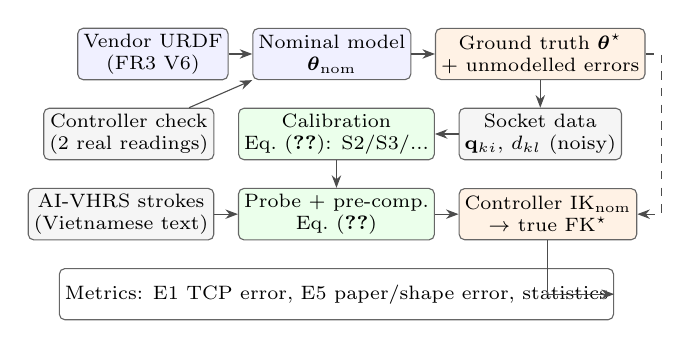
\begin{tikzpicture}[font=\scriptsize, node distance=3.5mm and 3mm,
  box/.style={draw=black!60, rounded corners=2pt, align=center, minimum height=6.5mm, inner sep=2pt, fill=#1},
  box/.default=white, arr/.style={-{Stealth[length=1.6mm]}, black!70}]
\node[box=blue!6] (urdf) {Vendor URDF\\(FR3 V6)};
\node[box=blue!6, right=of urdf] (nom) {Nominal model\\$\boldsymbol\theta_{\rm nom}$};
\node[box=orange!10, right=of nom] (truth) {Ground truth $\boldsymbol\theta^\star$\\+ unmodelled errors};
\node[box=gray!8, below=of truth] (sock) {Socket data\\$\mathbf q_{ki}$, $d_{kl}$ (noisy)};
\node[box=green!8, left=of sock] (cal) {Calibration\\Eq.~(\ref{eq:J}): S2/S3/...};
\node[box=gray!8, left=of cal] (ctrl) {Controller check\\(2 real readings)};
\node[box=green!8, below=of cal] (pc) {Probe + pre-comp.\\Eq.~(\ref{eq:pc})};
\node[box=gray!8, left=of pc] (txt) {AI-VHRS strokes\\(Vietnamese text)};
\node[box=orange!10, right=of pc] (exe) {Controller IK$_{\rm nom}$\\$\to$ true FK$^\star$};
\node[box=white, below=of pc] (met) {Metrics: E1 TCP error, E5 paper/shape error, statistics};
\draw[arr] (urdf) -- (nom); \draw[arr] (nom) -- (truth); \draw[arr] (truth) -- (sock);
\draw[arr] (sock) -- (cal); \draw[arr] (cal) -- (pc); \draw[arr] (txt) -- (pc); \draw[arr] (pc) -- (exe);
\draw[arr] (exe) |- (met); \draw[arr] (ctrl) -- (nom.south west);
\draw[arr, dashed] (truth.east) -- ++(2mm,0) |- (exe.east);
\end{tikzpicture}
\caption{Research pipeline. Orange: simulated physical robot (never visible to the calibration). Green: the evaluated methods.
The nominal model is checked against real controller readings; everything downstream is simulated.}
\label{fig:arch}
\end{figure}

\subsection{Robot and nominal model}
The nominal model is the vendor URDF of the FR3 V6 \cite{frcoburdf} (the robot in the AI-VHRS workshop: FR3 V6.0,
controller V3.8.25-QX). Our NumPy forward kinematics agrees with PyBullet \cite{pybullet} on the same URDF (through the
AI-VHRS robot-agent module) to within $7.6\times10^{-4}$\,mm over 2000 random configurations. Two read-only readings
of the real controller (joint angles and reported flange pose) are reproduced by the URDF chain plus a 100\,mm flange
offset along the last joint axis (fitted 99.9997 and 100.0019\,mm) with residuals of 0.011 and 0.009\,mm and
0.0005\,$^\circ$. This validates the controller's \emph{nominal} model, not the robot's true accuracy.

\subsection{Scene}
The paper corners are the three pen-tip probe points recorded in the AI-VHRS workcell (A4 portrait); the pen tip is
179.62\,mm from the flange (the workshop's current tool; its direction is assumed along the flange axis); the writing
orientation is the real pen-down flange orientation, re-aligned with the sheet normal. The calibration ball is assumed at
the pen position. Sockets are 12\,mm above the sheet, centred on it, spacing $d=150$\,mm.

\subsection{Ground-truth robots and uncertainties}
Each trial draws an independent ground-truth robot (Table~\ref{tab:sim}). Besides geometric deviations in the calibrated
parameter space, the truth contains two error sources \emph{outside} the model class: a periodic joint transmission error and
gravity-induced joint compliance with a lumped-mass model (URDF link masses) and assumed joint stiffness. The calibration
receives only noisy joint readings, cluster labels and measured distances; a unit test enforces this. Calibration
configurations are drawn by tilting the tool up to $\alpha=30^\circ$ from the sheet normal (the only freedom of a 6-DOF arm
with the ball pinned) and spinning it $\pm60^\circ$, rejecting draws outside joint limits minus $5^\circ$ (rejected draws are
logged: 0 for S2, 81 for S3 and 109 for S2$\times$2 over 30 trials).

\begin{table}[t]
\caption{Simulation parameters (all are assumptions unless a source is given)}\label{tab:sim}
\centering\scriptsize
\setlength{\tabcolsep}{3pt}
\begin{tabular}{@{}lll@{}}
\toprule
Quantity & Value & Basis\\
\midrule
Joint-origin translation dev. & $\mathcal N(0,0.5^2)$ mm & assumed\\
Joint-origin rotation dev. & $\mathcal N(0,0.1^2)$ deg & assumed\\
Transmission error amplitude & $\mathcal U(0,0.003)$ deg & assumed\\
Joint stiffness $K_{1\ldots6}$ & 30,30,20,10,10,10 kN\,m/rad & assumed\\
Link masses / payload & URDF / 0.6 kg & URDF / assumed\\
Ball, pen offset error & $\mathcal N(0,0.3^2)$ mm/axis & assumed\\
Socket seating noise (std) & 0.02 mm & assumed\\
Encoder noise (std) & 0.001 deg & assumed\\
Socket distance error (std) & 0.02 mm & assumed\\
Probing error, in-plane/normal & 0.10 / 0.02 mm & assumed\\
Tilt cone / spin range & 30 / $\pm$60 deg & design\\
Calibration samples $N$ & 60 & MUKCa: $\geq$30/socket\\
Regularisation $\lambda$ & $10^{-4}$ & MUKCa\\
Paper corners, pen offset & workcell values & AI-VHRS files\\
\bottomrule
\end{tabular}
\end{table}

\subsection{Dataset}
Ten writing samples on the A4 sheet: three straight lines (170--308\,mm), four small circles ($r=5$\,mm) at the sheet
corners, one large circle ($r=80$\,mm), a square and a zig-zag (corners), eight Vietnamese characters with stacked diacritics (breve, circumflex or horn
combined with a tone mark, and the barred d), three words, a short sentence (``Xin ch\`ao Vi\d{\^e}t Nam\ldots''),
and a full paragraph of Vietnamese text (632 strokes, 4.9\,m of path). Text trajectories are \emph{font-generated} by the
AI-VHRS OT-3 composer (public-domain single-line Hershey glyphs with hand-designed Vietnamese diacritic strokes); they are not
recorded human handwriting, and no human ground-truth trajectories are used. Paths are resampled every 1\,mm (9321 points per
trial and method).

\subsection{Protocol and baselines}
\textbf{E1} (calibration accuracy): 30 ground-truth robots; for each, nominal, S2, S3L, S2$\times$2 and S3 models are
evaluated on the same independent test set of 500 true configurations spread over the sheet, 0--60\,mm above it, tilted up
to $20^\circ$. \textbf{E5} (handwriting): the same 30 robots; methods A (nominal model, sheet pose known exactly, no
probing), B (nominal model + probing; current AI-VHRS practice), C/E/D (S2 / S2$\times$2 / S3 calibration + probing +
pre-compensation) and O (oracle: true model + probing + pre-compensation; a lower bound set by probing noise). All methods
share the same robot, probe readings and test data (paired design). \textbf{E2}--\textbf{E4} (20 robots each): measurement
noise scaled $0$--$8\times$, unmodelled errors removed or doubled, geometric error scaled $0.5$--$4\times$, $\lambda$ ablation,
$N\in[12,150]$, socket spacing 50--250\,mm and tilt cone 5--45$^\circ$. Seeds are fixed and recorded. Statistics are computed
over robots (one value per robot), with bootstrap 95\% confidence intervals of the mean and two-sided Wilcoxon signed-rank tests
\cite{wilcoxon1945} with Holm correction \cite{holm1979}. No trial was excluded; all 1,950 E1/E5 rows (and 4,420 E2--E4
sensitivity rows) completed without solver or IK failure.

% =====================================================================================================================
\section{Experimental Results}
\begin{figure*}[t]
\centering
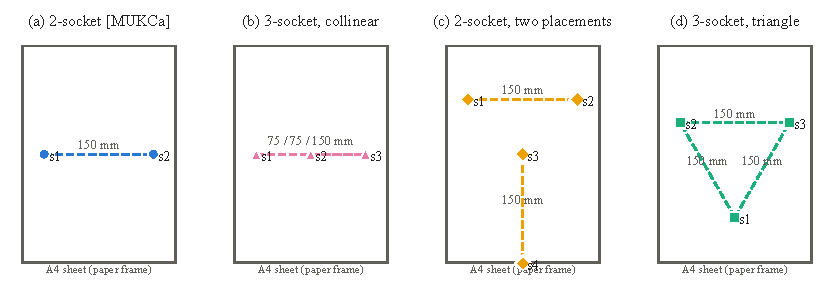
\includegraphics[width=\textwidth]{figures/fig2_socket_layouts.pdf}
\caption{Socket layouts in the paper frame (A4 sheet outline), all with $d=150$\,mm and the same total of $N=60$
configurations. (a) MUKCa two-socket tool; (b) three collinear sockets; (c) the two-socket tool at two placements; (d) the
proposed three-socket triangle. Dashed lines: pairs with a known distance.}
\label{fig:layouts}
\end{figure*}

\subsection{Identifiability (RQ1, RQ2)}
For all four layouts, all tilt cones from $2^\circ$ to $45^\circ$ and all ten robots, the rank of the identification
Jacobian was exactly 21 of 39, as predicted in Section~III-D. The 18 unidentifiable directions are the 6 base-gauge
parameters (verified to lie entirely in the null space) and 12 redundancies of the URDF parameterisation (e.g., translation
of joint 2 along the joint-1 axis). Hence a non-redundant 6-DOF arm \emph{does} supply enough configuration diversity
through tool orientation alone, and a third socket does not make additional parameters identifiable. The layouts differ in
how strongly the identifiable directions are excited (Table~\ref{tab:obs}): S3 and S2$\times$2 have a $1.6\times$ larger
$O_1$ and a $2.1\times$ larger geometric mean of the six weakest singular values than S2 and S3L.

\begin{table}[t]
\caption{Observability at $\alpha=30^\circ$, $N=60$ (median of 10 robots; singular values of the identification Jacobian,
parameters in mm/mrad)}\label{tab:obs}
\centering\scriptsize
\begin{tabular}{@{}lcccc@{}}
\toprule
Layout & rank & $O_1\,(\times10^{-3})$ & weakest-6 $(\times10^{-3})$ & $\sigma_{\min}\,(\times10^{-3})$\\
\midrule
\csname @@input\endcsname tables/table_obs.tex
\bottomrule
\end{tabular}
\end{table}

\subsection{E1: calibration accuracy (RQ1, RQ2)}
Table~\ref{tab:e1} and Fig.~\ref{fig:e1} summarise the 30 robots. The nominal model has a gauge-free TCP RMSE of
0.748\,mm (raw error 2.91\,mm including the base offset). MUKCa's two-socket layout reduces it by 85\% to 0.109\,mm; the
triangular three-socket layout reaches 0.044\,mm, a further 60\% reduction ($p_{\rm Holm}=5\times10^{-8}$, better in 28 of 30
robots). Three collinear sockets are indistinguishable from two ($p=0.78$), whereas the two-socket tool at two placements
reaches 0.049\,mm; the triangle is still 10\% better than S2$\times$2 ($p_{\rm Holm}=0.039$, 21/30 robots) and has the smallest
spread across robots (std 0.005\,mm). In all runs the solver converged (25--34 evaluations), the residual consistency was
0.038--0.040\,mm RMS and distances were matched within 0.004\,mm (0.037\,mm for S3L). Raw (non-aligned) errors remain
1.28--1.50\,mm because the base gauge is not observable from sockets; in the application it is removed by paper probing.
The identifiable part of the parameter error fell only to 52--67\% of its nominal value: the calibrated parameters absorb the
unmodelled compliance, so they are good predictors in the calibrated region but not the true geometry.

\begin{table}[t]
\caption{E1: TCP position error on an independent test set after rigid alignment (mm), mean over 30 simulated robots
($\pm$ std across robots; bootstrap 95\% CI of the mean RMSE)}\label{tab:e1}
\centering\scriptsize
\setlength{\tabcolsep}{2.5pt}
\begin{tabular}{@{}lccccc@{}}
\toprule
Model & MAE & RMSE & 95\% CI & P95 & max\\
\midrule
\csname @@input\endcsname tables/table_e1.tex
\bottomrule
\end{tabular}
\end{table}

\begin{figure}[t]
\centering
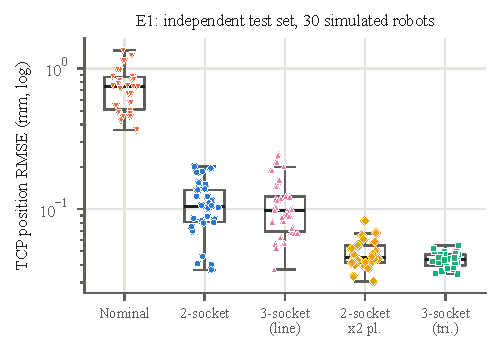
\includegraphics[width=\columnwidth]{figures/fig3_e1_calibration.pdf}
\caption{E1: per-robot TCP RMSE (log scale), 500 test configurations per robot, $N=60$ calibration samples for every layout.}
\label{fig:e1}
\end{figure}

\subsection{E5: handwriting accuracy (RQ3)}
Table~\ref{tab:e5} reports the means over 30 robots of the per-robot averages over the ten samples. Without probing (A),
the error is dominated by the robot's absolute error (2.52\,mm) and the pen lifts off the paper for 25\% of the path at a
0.3\,mm press depth (the depth currently configured in AI-VHRS). Probing with the nominal model (B) removes most of the offset
(0.80\,mm) and keeps full contact, but leaves the shape distortion unchanged (0.233\,mm), because probing only registers a
rigid frame. Calibration with pre-compensation reduces the absolute error to 0.18 (C), 0.145 (E) and 0.150\,mm (D), all
$p_{\rm Holm}<10^{-7}$ against B. D and E are not distinguishable from each other ($p=0.62$) or from the oracle O (0.141\,mm,
$p=0.62$): at this point the absolute error is limited by the probing uncertainty, not by the kinematic model. The shape
error separates the methods clearly: 0.037\,mm for C, 0.014\,mm for E and 0.010\,mm for D (D vs.\ C $-72\%$,
$p_{\rm Holm}=1.6\times10^{-7}$; D vs.\ E $-27\%$, $p_{\rm Holm}=0.007$). Fig.~\ref{fig:e5}(a,b) shows how the nominal error
grows across the sheet away from the probe points, and Fig.~\ref{fig:e5}(c) shows that the ranking holds for every sample;
large-scale figures (circles, diagonal line, corners) are the most distorted, single words the least.

\begin{table}[t]
\caption{E5: handwriting accuracy in the true paper frame (mm), mean over 30 robots of the per-robot average over ten samples
(9321 points per robot and method). Shape = in-plane error after the best 2-D rigid fit. Contact = path fraction with
$h<0.3$\,mm (geometric proxy). PC = pre-compensation.}\label{tab:e5}
\centering\scriptsize
\setlength{\tabcolsep}{2pt}
\begin{tabular}{@{}lccccccc@{}}
\toprule
Method & MAE & P95 & Chamfer & HD95 & Shape & $|h|_{\max}$ & Contact\,\%\\
\midrule
\csname @@input\endcsname tables/table_e5.tex
\bottomrule
\end{tabular}
\end{table}

\begin{figure*}[t]
\centering
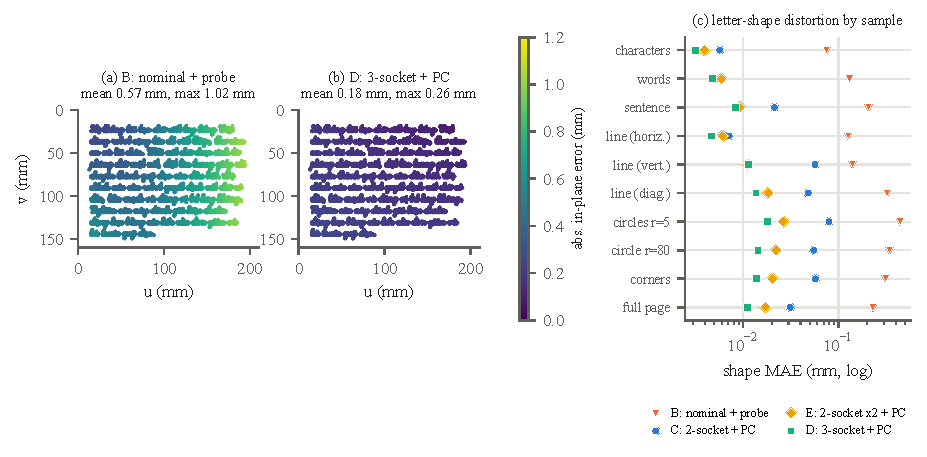
\includegraphics[width=\textwidth]{figures/fig4_e5_trajectories.pdf}
\caption{E5. (a,b) Absolute in-plane error along the full-page Vietnamese paragraph for one simulated robot (seed 1000):
nominal model with probing vs.\ three-socket calibration with pre-compensation. (c) Letter-shape distortion per sample, mean
over 30 robots (log scale).}
\label{fig:e5}
\end{figure*}

\textit{Failure cases.} In one robot (seed 1004), whose nominal model was already accurate (B shape error 0.067\,mm), S2
calibration slightly increased the shape error (0.073\,mm), whereas S3 reduced it (0.015\,mm). In one robot (seed 1021),
B had a lower absolute error (0.196\,mm) than D (0.253\,mm) and even the oracle (0.262\,mm): registration errors happened to
cancel part of the kinematic error. In E1, S3 was marginally worse than S2 in 2 of 30 robots (by $\leq0.005$\,mm).

\subsection{E2--E4: robustness, sample efficiency and geometry}
\begin{figure*}[t]
\centering
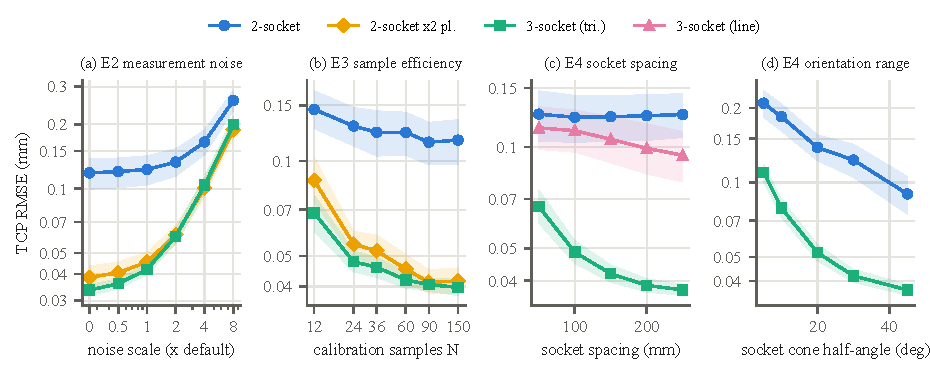
\includegraphics[width=\textwidth]{figures/fig5_sensitivity.pdf}
\caption{Sensitivity (20 robots per point; shaded: bootstrap 95\% CI of the mean). (a) Measurement noise (seating, encoder,
caliper) scaled from 0 to $8\times$ the default. (b) Number of calibration configurations. (c) Socket spacing. (d) Tool tilt
cone, the only source of configuration diversity for the 6-DOF arm.}
\label{fig:sens}
\end{figure*}
Fig.~\ref{fig:sens} shows: (a) the advantage of spread layouts holds up to $2\times$ the default noise and vanishes at
$4$--$8\times$ (S3 0.10 vs.\ S2 0.17\,mm at $4\times$; S3 0.20 vs.\ S2$\times$2 0.19\,mm at $8\times$), where noise dominates;
(b) S3 with only 12 configurations (0.068\,mm) beats S2 with 150 (0.116\,mm); (c) S2 does not improve with spacing
(0.123--0.125\,mm), S3L improves slowly and S3 improves from 0.067\,mm at 50\,mm to 0.038\,mm at 250\,mm; (d) a larger tilt
cone helps every layout (S3: 0.110\,mm at $5^\circ$, 0.037\,mm at $45^\circ$), and S3 at $10^\circ$ already beats S2 at
$45^\circ$. Halving the joint stiffness raised S3 to 0.064\,mm and S2 to 0.145\,mm. For geometric errors scaled $4\times$
(nominal 2.78\,mm), S3 kept 0.086\,mm while S2 reached 0.44\,mm; on the full page, B then lost pen contact on 21\% of the
path and reached 2.42\,mm MAE, versus 0.15\,mm for D.

\textit{Regularisation.} With noise-free data and no unmodelled errors, the S2 error was 0.107\,mm at $\lambda=10^{-4}$ but
$3\times10^{-4}$\,mm at $\lambda=10^{-8}$ (S3: 0.020 vs.\ $10^{-4}$\,mm); with default noise it was 0.088\,mm vs.\ 0.039\,mm for
S3 at $\lambda=10^{-8}$. Thus, at MUKCa's $\lambda$, part of the S2 deficit is regularisation bias along weakly excited
directions, and the remainder is noise amplification along the same directions; both shrink with the larger $O_1$ of spread
layouts. $\lambda=10^{-6}$ was better than $10^{-4}$ for every layout in our setting (S3 0.039, S2 0.084\,mm); the main
results keep MUKCa's value because no ground truth is available to tune $\lambda$ on a real robot.

% =====================================================================================================================
\section{Discussion}
\textit{Why three sockets help, and when.} The third socket does not add identifiable parameters; it enlarges the weakest
excited directions by spreading the constraints over the plane. The evidence is consistent across four independent views:
the collinear control (no gain), the two-placement control (almost the same gain), the observability index (same ordering)
and the spacing study (S3 improves with spread, S2 does not). The practical answer to RQ2 is therefore: a triangular socket
tool is preferable when only one placement is possible and measurement noise is at most about twice our assumed level;
otherwise, relocating a two-socket tool once achieves most of the benefit. The triangle has the extra practical advantage of
one fixture and one set of distance measurements.

\textit{Transfer to a 6-DOF arm.} MUKCa's redundancy assumption is not needed for identifiability when the end effector
pivots in a spherical socket: tilting and spinning the tool provides full rank even at $2^\circ$ of tilt, but accuracy
degrades for small cones (Fig.~\ref{fig:sens}d). Whether the physical FR3 can be hand-guided through a $30^\circ$ cone with the
ball seated, without reaching joint limits or table collisions of the gripper, must be checked on the robot.

\textit{What the handwriting application needs.} Probing alone already removes most of the absolute offset, so the visible
benefit of calibration is in letter shapes over the sheet (0.233 to 0.010\,mm) and in robustness when the robot is less
accurate (geometric errors $4\times$: contact loss with B, none with D). Absolute placement is limited by probing
(0.14\,mm for a perfect model), which suggests probing more points or using a probing jig as the next improvement.

\textit{Limitations.} (1) All results are simulated; the error magnitudes of Table~\ref{tab:sim} are assumptions, not
measurements of the workshop FR3, so absolute numbers may not transfer, while the relative conclusions were stable across
the ranges of E2--E4. (2) The controller is modelled as exact IK of the nominal model; trajectory interpolation, dynamics,
servo tracking, latency and backlash are not modelled (MUKCa reports backlash as a failure mode \cite{franzese2026mukca}).
(3) Compliance during hand-guiding (contact forces in the socket) and a non-rigid gripper are not modelled. (4) The text
trajectories are font-generated, not human handwriting, and ink deposition, pen force and paper deformation are not
simulated; contact ratio is a geometric proxy. (5) The ground truth shares the URDF parameterisation for its geometric part;
the unmodelled terms mitigate, but do not remove, this ``inverse crime''. (6) The ball offset direction and the pen-tool
direction were assumed.

% =====================================================================================================================
\section{Conclusion and Future Work}
In simulation, MUKCa-style socket calibration transfers to the non-redundant 6-DOF FR3: the identifiable rank (21/39) is the
theoretical maximum for base-free position data, and calibration reduced the gauge-free TCP RMSE from 0.75\,mm to 0.11\,mm
with two sockets and 0.044\,mm with a triangular three-socket layout at equal sample count. The improvement comes from
two-dimensional socket spread, which a relocated two-socket tool also provides. Combined with joint-space pre-compensation
through the closed controller and paper probing, it reduced Vietnamese letter-shape distortion from 0.233 to 0.010\,mm and
absolute in-plane error from 0.80 to 0.15\,mm. Future work: build the socket tool and hand-guide the real FR3 through it;
measure the true TCP error with an external reference to validate the simulated gains; verify that the controller's
inverse kinematics reproduces the joint solution of Eq.~(\ref{eq:pc}); and evaluate ink-on-paper quality with the AI-VHRS
photo-based evaluator.

\section*{Acknowledgment}
[To be completed by the authors.] Draft prepared with AI assistance; the authors are responsible for verifying all content
before any submission, in line with the target venue's policy on AI-generated text.

\bibliographystyle{IEEEtran}
\bibliography{references}

\end{document}
